\documentclass[output=paper]{langsci/langscibook} 
\author{Holger Diessel\affiliation{Please provide affiliation}}
\title{Preposed adverbial clauses: Functional adaptation and diachronic inheritance}
\abstract{In the historical literature it is commonly assumed that subordinate clauses are derived from paratactic sentences. However, while this assumption is not implausible for certain types of postposed adverbial clauses, there is no obvious connection between preposed adverbial clauses and parataxis. This paper investigates the diachronic development of preposed adverbial clauses from a cross-linguistic perspective. Drawing on data from a typological and diachronic database, it is shown that preposed adverbial clauses evolve from various diachronic sources that are semantically and structurally similar to the target construction (e.g. adpositional phrases, pre- and postnominal relative clauses, juxtaposed sentences). Considering the factors behind these developments, the paper argues that while the occurrence of preposed adverbial clauses can be explained by general cognitive processes of language use, the internal structure of preposed adverbial clauses, notably the position of the subordinator, is primarily determined by grammaticalization.}
\begin{document}
\maketitle 

 

\section{Introduction}

It is a standard assumption of historical linguistics that syntactic structures often develop from structurally independent elements in discourse \citep{Givón1979}. An oft-cited example is the diachronic development of subordinate clauses from paratactic sentences. As \citet{Lehmann1988} and others have shown, there is a cline of clause linkage ranging from the combination of two structurally independent sentences in discourse to tightly organized bi-clausal structures in which one clause is syntactically dependent on the other one. Building on this observation, it is commonly assumed that subordinate clauses have evolved from independent sentences or parataxis (e.g. \citealt{HopperTraugott2003}: 176--184). However, while this assumption appears to be plausible for many postposed subordinate clauses, there is no obvious connection between parataxis and preposed subordinate clauses.

Clause combining in discourse has a backwards orientation. Paratactic sentences are usually related to previous sentences, as evidenced by the occurrence of anaphoric pronouns and clause linkers that connect the current sentence to participants and propositions of the preceding sentence or discourse (cf. (1)).
 

\ea\label{ex:key:}

\textit{Jo\tikzmark{john}{\vphantom{fj}}hn\textsubscript{i}} was accepted to Harvard.\tikzmark{fullstop}{} \textit{There\tikzmark{f}{}fore, h\tikzmark{he}{\vphantom{fj}}e\textsubscript{i}} moved to Boston.\\ 

\begin{tikzpicture}[overlay,remember picture]
  \node (h2) [below=0mm of he] {};
  \node (john2) [below=0mm of john] {};
  \draw[thick,dotted] (he) -- (h2.south);
  \draw[thick,dotted] (h2.south) -- (john2.south);
  \draw[thick,dotted,-latex] (john2.south) -- (john);
  \draw[thick,dashed,Circle-latex,transform canvas={yshift=3mm}] (f.north) --   (fullstop.north);
  
% \draw[dashed,rounded corners]   (x5.south) |- (A3.east) ;
\end{tikzpicture}
\z

% \draw circle [radius=#1];


Like independent sentences, complex sentences are processed with a backwards orientation if the subordinate clause follows the main clause (e.g. \textit{John\textsubscript{i}} \textit{moved} \textit{to} \textit{Boston,} \textit{because} \textit{he\textsubscript{i}} \textit{was} \textit{accepted} \textit{to} \textit{Harvard}). However, unlike paratactic sentences, preposed subordinate clauses have an inherent forward orientation in that pronouns and clause linkers are related to elements of the upcoming main clause (cf. (2)).

 
\begin{figure}
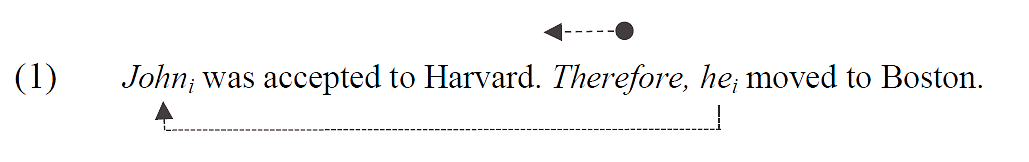
\includegraphics[width=\textwidth]{figures/diessel-img1.png}
\end{figure}


%%[Warning: Draw object ignored]

\ea\label{ex:key:}
\ea%2
    \label{ex:key:2} Because \textit{he\textsubscript{i}} was accepted to Harvard, \textit{John\textsubscript{i}} moved to Boston. 
  \z
  \z
  
\begin{figure}
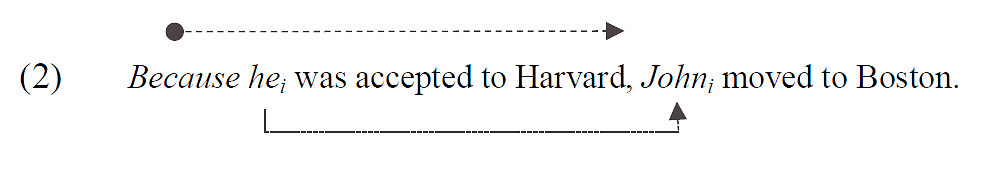
\includegraphics[width=\textwidth]{figures/diessel-img2.png}
\end{figure}

Considering the projective force of preposed subordinate clauses, it is unclear if and how these structures have evolved from clause combining strategies in discourse. It is the purpose of this paper to investigate the diachronic developments of preposed subordinate clauses from a cross-linguistic perspective. Specifically, the paper is concerned with the development of preposed adverbial clauses. 

Following \citet{Cristofaro2003}, adverbial clauses are here defined as part of a biclausal construction consisting of a main clause and a subordinate clause in which the event designated by the subordinate clause specifies the circumstances under which the event of the main clause takes place. Several typological studies have investigated the positional patterns of adverbial clauses (e.g. \citealt{Greenberg1963,Diessel2001}; Schmidtke-\citealt{Bode2009,DiesselHetterle2011,Hetterle2015}); but they are either based on small and biased samples or concentrate on particular adverbial relations (e.g. purpose or cause). In the current study, we will be concerned with four general semantic types of adverbial clauses (i.e. adverbial clauses of time, condition, cause and purpose) based on data from a genetically and geographically dispersed convenience sample of 100 languages. The languages come from 85 genera (which maximally include two languages) and six large geographical areas (i.e. Eurasia, Africa, South East Asia and Oceanic, Australia and New Guinea, North America, South America) (cf. \citealt{Dryer1992}). The bulk of the data were gathered from reference grammars and other published sources, supplemented by information from native speakers and language specialists.\footnote{A list of languages included in the sample is given in the Appendix.} 

The paper is divided into three parts. The first part describes the cross-linguistic distribution of preposed adverbial clauses in the 100 language sample; the second part provides an overview of the main diachronic paths to preposed adverbial clauses; and the third part considers the developments described in light of the debate about functional and diachronic explanations for language universals that takes center stage in the present volume.

\section{Cross-linguistic patterns}

Let us begin with some general observations regarding the position of subordinate clauses. Subordinate clauses are dependent categories of an associated element. Three basic types of subordinate clauses are commonly distinguished: 
(i) complement clauses, which are dependent categories of a complement-taking verb or predicate, 
(ii) relative clauses, which are dependent categories of a noun or noun phrase, and 
(iii) adverbial clauses, which may be seen as dependent categories of a main clause or main clause predicate. 

The position of all three types of subordinate clauses relative to the associated element correlates with the position of other dependent categories relative to the so-called head, but the correlations are skewed in particular directions \citep{Diessel2001}. As \citet{Greenberg1963} already noted, the order of relative clause and noun correlates with that of verb and object, but there is a predominance of postnominal relative clauses. In VO languages, relative clauses are almost always postposed to the associated N(P), but in OV languages we find both pre- and postnominal relatives (cf. \citealt{Dryer2005}). 

The order of complement clause and verb is similar. As Schmidtke-\citet{BodeDiessel2017} have shown, although object complement clauses usually serve the same syntactic function as object NPs, they do not always occur in the same structural position as nominal objects. In VO languages, complement clauses follow the verb with almost no exception, but in many OV languages they are postposed to the main verb, as for instance in Persian, Epena Pedee and Supyire. There is thus a general tendency for both relative and complement clauses to follow the associated category, which may be due to the oft-noted trend for long and heavy constituents to follow short ones (cf. \citealt{Behaghel1932}).

However, adverbial clauses are different. Although adverbial clauses are long constituents, they often precede the main clause. As \citet{Diessel2001} observed (based on data from a small and biased sample), in VO languages, adverbial clauses occur both before and after the associated main clause, but in some OV languages, there is a general tendency to prepose all adverbial clauses. This tendency is also evident in the current sample (cf. \tabref{tab:key:1}).

\begin{table}
\small
\begin{tabularx}{\textwidth}{lSSSr}
\lsptoprule
&   Languages in which all types of ACs (usually) precede the MC &   Languages in which ACs are commonly pre- and postposed &   Languages in which all types of ACs (usually) follow the MC &   Total\\
\midrule 
VO & - & 40 & - & 40\\
VO/OV & - & 8 & - & 8\\
OV & 31 & 21 & - & 52\\
\midrule
Total & 31 & 69 & - & 100\\
\lspbottomrule
\end{tabularx}

\caption{The position of adverbial clauses and the order of verb and object}
\label{tab:diessel:1}
\end{table}

As can be seen, most of the languages of the current sample make common use of both pre- and postposed adverbial clauses, but in more than half of all OV languages, adverbial clauses are usually preposed to the main clause. In Japanese, for instance, there is a very strong tendency to prepose adverbial clauses (though in spoken Japanese, adverbial clauses sometimes follow the main clause as afterthoughts; cf. \citealt{FordMori1994}).

Generalizing across the data in \tabref{tab:key:1}, we may say that while the order of adverbial clause and main clause correlates with that of verb and object, the occurrence of preposed adverbial clauses is cross-linguistically predominant. However, on closer inspection we find that the predominance of preposed adverbial clauses is mainly due to certain semantic types of adverbial clauses that precede the main clause in both VO and OV languages. Consider the data in \tabref{tab:key:2}, which show that the positional patterns of adverbial clauses correlate with their meaning.  

\begin{table}
\begin{tabularx}{\textwidth}{Xrrrr} 
\lsptoprule
&   Preposed &   Pre- and postposed &   Postposed &   Total\\
\midrule
Condition & 94 [91.3\%] & 9 [8.7\%] & 0 [0\%] & 103\\
Time & 119 [59.8\%] & 68 [34.2\%] & 12 [6.0\%] & 199\\
Cause & 40 [38.8\%] & 24 [21.2\%] & 49 [43.4\%] & 113\\
Purpose & 33 [28.7\%] & 19 [16.5\%] & 63 [54.8\%] & 115\\
\midrule 
Total & 286 & 120 & 124 & 530\\
\lspbottomrule
\end{tabularx}

\caption{The meaning and position of adverbial clause constructions in a sample of 100 languages}
\label{tab:diessel:2}
\end{table}

Note that the frequencies in \tabref{tab:key:2} are based on constructions rather on languages. Since some languages have multiple adverbial clause constructions of the same semantic type, \tabref{tab:key:2} includes a larger number of constructions than languages. Note also that this table concerns both adverbial clauses that are tied to a specific position by linguistic convention and adverbial clauses that are statistically biased to precede or follow the main clause. In the latter case, some of the data in \tabref{tab:key:2} are based on frequency counts from linguistic corpora, but more often these data are based on field workers’ judgements regarding the position of adverbial clauses. While expert judgements are less reliable than corpus counts, they provide a reasonable estimate as to how main and adverbial clauses are arranged in a particular language.\footnote{Psycholinguistic evidence suggests that while speakers have difficulties to estimate the absolute frequencies of linguistic elements, their judgements of relative linguistic frequencies are quite reliable (\citealt{HasherZacks1984}).}

As can be seen, conditional clauses typically precede the main clause (cf. \citealt{Greenberg1963}: Universal 14), though in many languages, conditional clauses can also be postposed to the main clause. Like conditional clauses, temporal clauses tend to precede the main clause, but temporal clauses follow the main clause more often than conditionals. The position of temporal clauses varies with the nature of the temporal link they encode. For instance, temporal clauses denoting a prior event, i.e. an event that precedes the one in the main clause, are more often preposed than temporal clauses denoting a posterior event. In English, for example, \textit{after}- and \textit{since}-clauses denote a prior event and precede the main clause more often than adverbial clauses denoting a posterior event such as \textit{before}- and \textit{until}-clauses (cf. \citealt{Diessel2008}). The same tendency has been observed in several other languages of the current sample (e.g. in German, Supyire, Abun, Nkore Kiga, Noon, and Taba). 

Moreover, and this is particularly striking, there is a general tendency to prepose adverbial clauses that correspond to English \textit{when}-clauses. Like \textit{after} and \textit{since}, \textit{when} can denote a prior event, but it can also indicate a link between events that occur simultaneously \citep{Diessel2008}. However, regardless of the temporal relationship that is expressed by a \textit{when}-clause, there is a tendency for temporal \textit{when}-clauses to precede the main clause. In fact, in a substantial number of languages \textit{when}-clauses are generally preposed to the main clause in the current sample (i.e. Abun, Supyire, Yagua, Trumai, Motuna). 

Finally, cause and purpose clauses tend to follow the main clause. \tabref{tab:key:2} shows that there are 40 adverbial clause constructions of cause and 33 adverbial clause constructions of purpose that precede the main clause, but most of these constructions occur in languages like Japanese, in which all adverbial clauses are preposed to the main clause regardless of their meaning. Generalizing across these findings we may conclude that that the cross-linguistic tendency to prepose adverbial clauses is mainly due to the fact that conditional clauses and certain types of temporal clauses, notably \textit{when}-clauses, precede the main clause regardless of the order of other syntactic constituents.

Interestingly, a number of studies suggest that the position of adverbial clauses does not only correlate with the semantic link between main and adverbial clauses, but also with aspects of their internal structure. Of particular importance is here the position of the subordinator (cf. \citealt{Diessel2001}; Schmidtke-\citealt{Bode2009,Hetterle2015}). Across languages, adverbial clauses are often marked by subordinate conjunctions that typically appear at the beginning or end of the subordinate clause. \citet{Dryer1992} showed that the position of the subordinator correlates with the order of verb and object: In VO languages, adverbial clauses usually occur with initial subordinators, but in OV languages they often include a final marker. However, the position of the subordinator does not only correlate with the order of verb and object, it also correlates with the position of the adverbial clause. Consider the data in \tabref{tab:key:3}, which is restricted to adverbial clauses with free subordinating morphemes.\footnote{Since adverbial clause constructions that do not include a free subordinating morpheme are disregarded, \tabref{tab:key:3} includes only a subset of the adverbial clause constructions in \tabref{tab:key:2}.} 

\begin{table}
\begin{tabularx}{\textwidth}{X rr p{1mm} rr p{1mm} rr  @{}p{0mm}r}
\lsptoprule
& \multicolumn{2}{p{2cm}}{\centering ~\\  Preposed} &&
  \multicolumn{2}{p{2.5cm}}{\centering  Flexible\newline (no preference)} && 
  \multicolumn{2}{p{2cm}}{\centering ~\\Postposed} &    \\
\cmidrule{2-3}\cmidrule{5-6}\cmidrule{8-9}
&   Initial &   Final &&   Initial &   Final &&   Initial &   Final && Total\\
\midrule
{condition} 	& 34 	& 22 	&& 5 	& - 	&& - 	& - 	&& 61\\
{time} 		& 20 	& 47 	&& 43 	& 5 	&& 7 	& 3 	&& 125\\
{cause} 	& 2 	& 26 	&& 11 	& 6 	&& 37 	& 4 	&& 86\\
{purpose} 	& - 	& 20 	&& 2 	& 4 	&& 38 	& 4 	&& 68\\
\midrule
{total} 	& 56 	& 115 	&& 61 	& 15 	&& 82 	& 11 	&& 340\\
\lspbottomrule
\end{tabularx}

\caption{The position of free subordinators in pre- and postposed adverbial clauses}
\label{tab:diessel:3}
\end{table}

As can be seen, adverbial clauses that follow the main clause or that are flexible with regard to their position typically occur with an initial marker. There are languages in which postposed and flexible adverbial clauses include a final marker, but this is relatively rare (and mainly found in certain areas, e.g. South America). By contrast, preposed adverbial clauses are frequently marked by a final subordinator, especially in languages in which all adverbial clauses precede the main clause, as for instance in Amele, Burmese, Japanese, Korafe, Korean, Santali, Slave, Turkish, Wappo, Warao, and Menya. Only conditional clauses and temporal \textit{when}-clauses are commonly preposed and often marked by an initial subordinator (in languages in which other semantic types of adverbial clauses are flexible or postposed to the main clause). 

\section{Diachronic sources}

Having described the positional patterns of adverbial clauses (and adverbial subordinators), let us now consider their diachronic evolution. Where do preposed adverbial clauses come from? In the historical literature, syntactic development is commonly described as a process that leads from a source construction A to a target construction B, but this scenario is not always appropriate to characterize syntactic change (cf. \citealt{Givón1991}; Van de \citealt{VeldeEtAl2013}). Since subordinate clauses are complex grammatical units, they are usually related to several other constructions, e.g. other types of subordinate clauses, certain types of phrasal constituents and independent sentences. Since all of these constructions can influence the development of a particular adverbial clause, it is not always possible to trace adverbial clauses to one specific source. However, while the diachronic developments of adverbial clauses are (usually) influenced by several constructions, in many cases there is one construction that is so closely related to a certain type of adverbial clause that it can be seen as the primary determinant, or source, of that clause. For instance, many postposed adverbial clauses are so similar to paratactic sentences that it seems reasonable to assume that parataxis has a significant impact on the development of (many) postposed subordinate clauses. However, while the development from parataxis provides a plausible scenario for the rise of (many) postposed adverbial clause, it does not explain where preposed adverbial clauses come from.

Since preposed adverbial clauses are thematically related to the ensuing discourse, there is no obvious connection to parataxis unless we assume that preposed adverbial clauses are based on postposed subordinate clauses that were fronted after they developed from paratactic sentences. However, there is no evidence for this scenario. The diachronic developments of adverbial clauses have been examined in a large number of studies (e.g. \citealt{Haiman1985,Haspelmath1989,Givón1991,Genetti1991,HarrisCampbell1995,Frajzyngier1996,DisterheftViti2010}), but although fronting appears to provide a plausible scenario for the development of preposed adverbial clauses, there is almost no evidence for this scenario in the historical literature. On the contrary, what previous studies suggest is that adverbial clauses usually occur in the same position as their diachronic sources. In what follows, we consider four common source constructions for preposed adverbial clauses.

First, while preposed adverbial clauses are unlikely to have evolved from paratactic sentences through fronting, there is one common diachronic path that leads from independent sentences in discourse to complex sentences with preposed adverbial clauses. As \citet[39--70]{Haiman1985} observed, in many languages conditional relations are expressed by juxtaposed clauses that have the same structure as two simple sentences, as in the following examples from Vietnamese (cf. (3)), Mapudungun (cf. (4)) and Wambaya (cf. (5)).

\ea\label{ex:key:}
\langinfo{Vietnamese}{Austro-Asiatic, Viet-Muong}{\citealt{Haiman1985}: 45}\\
\gll  [Không  có   màn],  không  chịu  nôi.\\
       not  be   net  not  bear  can\\
\glt   `If there’s not net, you can’t stand it.'
\z

\ea\label{ex:key:}
\langinfo{Mapudungun}{Araucanian}{\citealt{Smeets2008}: 184}\\
\gll   [Aku-wye-fu-l-m-i],    pe-pa-ya-fwi-y-m-i.\\
       arrive-\textsc{plpf}-\textsc{ipd}-\textsc{cond}-2-\textsc{sg}  see-hither-\textsc{irr}-\textsc{obj}-\textsc{ind}-2-\textsc{sg}\\
\glt   `If you had arrived (by then), you would have seen him.'
\z

\ea\label{ex:key:}
\langinfo{Wambaya}{West Barkly}{\citealt{Nordlinger1998}: 219}\\
\gll   [Yabu  ng-uda  gijilulu]            jiyawu  ng-uda.\\
       have    \textsc{1sg}.\textsc{a-nact.pst}  money.\textsc{iv(acc)}  give  1\textsc{sg.a-nact.pst}\\
\glt   `If I’d had the money I would have given (it to her).'
\z

While some of these languages have conditional markers (e.g. Vietnamese \textit{nêu} ‘if’), conditional relations are commonly expressed by unmarked sentences that have the same structure as main clauses: they include finite verb forms, occur with the same arguments and adjuncts as independent sentences, and do not include an (obligatory) subordinate marker. Note, however, that while these constructions look like independent sentences, they are intonationally bound to the ensuing clause and sometimes constrained with regard to verb inflection. The conditional clause in Mapudungun, for instance, takes a mood suffix that is optional in main clauses but obligatory in conditionals. Moreover, in some languages these constructions occur with a topic or focus marker that one might analyze as a subordinator, such as the focus clitic at the end of the protasis in example (6) from Mangarayi.

\ea\label{ex:key:}
\langinfo{Mangarayi}{Isolate}{\citealt{Merlan1982}: 22}\\
\gll   [Na-yang-gu=\textbf{bayi}]   wawg   wa-nan-mi  biwin-gana.\\
       \textsc{2sg}-go-\textsc{des-foc}    follow   \textsc{irr-1sg>2sg-aux}  behind-\textsc{abl}\\
\glt   `If you go, I will follow (after) you.'
\z

In addition to conditional clauses, preposed temporal clauses are sometimes based on juxtaposed sentences (e.g. Lao, Vietnamese, Taba, Tetun, Gooniyandi); but preposed cause and purpose clauses are usually based on other types of constructions. Adpositional phrases, for instance, are often closely related to (preposed) cause and purpose clauses. Consider, for instance, the following examples from Turkish (cf. (7)) and Amele (cf. (8)), in which cause and purpose clauses are marked by benefactive postpositions. 

\ea\label{ex:key:}
\langinfo{Turkish}{Turkic}{\citealt{Kornfilt1997}: 74}\\
\gll   Hasan   [kitab-ı  san-a  ver-diğ-im  \textbf{için}]  çok  kız-dı.\\
       Hasan  book-\textsc{acc}  you-\textsc{dat}  give-\textsc{f.nml-1sg}  for  very  angry-\textsc{pst}  \\
\glt   `Hasan got very angry because I gave the book to you.'
\z

\ea\label{ex:key:}
\langinfo{Amele}{Nuclear Trans New Guinea, Madang}{\citealt{Roberts1987}: 58}\\
\gll   [Ija    sab    faj-ec   \textbf{nu}]  h-ug-a.\\
       \textsc{1sg}   food   buy-\textsc{inf/noml}  for  come-\textsc{1sg-pst}\\
\glt   \textsc{“}I came to buy food.'
\z

Note that the adverbial clauses in both examples are expressed by nominalizations. While adpositions and case affixes are also found with finite clauses, they are especially frequent with nominalized clauses, suggesting that nominalization provides a link between adpositional phrases and fully developed (subordinate) clauses (cf. \citealt{Deutscher2009,Heine2009}).

Adverbial clauses that are morphologically related to adpositional phrases are widely used to express semantic relations of cause and purpose. In addition, certain types of temporal clauses denoting a prior or posterior event are often strikingly similar to (temporal) adpositional phrases (e.g. Engl. \textit{after-,} \textit{since-} and \textit{before}-clauses) (\citealt{Blake1999,Hetterle2015}); but conditional clauses and temporal \textit{when}-clauses are only rarely marked by adpositions. 

Apart from juxtaposed sentences and adpositional phrases, relative clauses provide a very frequent source for (preposed) adverbial clauses. The development is well-known from English. As \citet{HopperTraugott2003} have shown, temporal \textit{while}-clauses have evolved from a relative or appositive construction that modified a generic head noun meaning ‘time’ (cf. (9)).

\ea\label{ex:key:}
\langinfo{Old English}{Indo-European, Germanic}{\citealt{HopperTraugott2003}: 90}\\
\gll   \& wicode    Þær   Þa   \textbf{hwile}  [Þe   man  Þa   burg  worthe  \& getimbrode].\\
       and  lived   there   that.\textsc{dat}   time.\textsc{dat}  that   one  that   fortress  worked.on  and built\\
\glt “… and camped there at the time that/while the fortress was worked on and built.'
\z

Similar types of adverbial clauses occur in many other languages of the current sample (e.g. in Mayogo (ex. (10)) and Toqabaqita (ex. (11)). Sometimes the subordinator is based on a generic noun, and sometimes it is based on a relative marker (as for instance many of the adverbial subordinators in Tamashek; cf. \citealt{Heath2005}: 660). 

\ea\label{ex:key:}
\langinfo{Mayogo}{Niger-Congo, Ubangi}{\citealt{Sawka2001}: 153}\\
\gll   [\textbf{Nedhinga}  u   a-zu   ‘he],   ndili-e   a-si   kuto.\\
        \textbf{while} (=time)  \textsc{3pl}   \textsc{pst-}eat   thing   child-\textsc{ref}   \textsc{pst-}sleep   down\\
\glt   `While they ate something, this child slept on (the) floor.'
\z

\ea\label{ex:key:}
\langinfo{Toqabaqita}{Austronesian, Oceanic}{\citealt{Lichtenberk2008}: 1173}\\
\gll   [\textbf{Si}   \textbf{manga}  \textbf{na}   kero  fula  mai],  keko  qono  qa-daroqa …\\
        \textsc{prtt}   time  \textsc{rel}   3\textsc{du.non.fut}  arrive  \textsc{vent}  \textsc{3du.seq}  sit  \textsc{sben-3du.pers}\\
\glt   `When (lit. ‘the time that’) they arrived, they sat (down)…”
\z

The development is especially frequent with temporal \textit{when}- and \textit{while}-clauses, but there are also other semantic types of adverbial clauses that are based on relative clauses in my data. In German, for instance, cause and condition clauses are marked by adverbial subordinators (i.e. \textit{weil} and \textit{falls}) that are based on nominal heads of relative or appositive clauses meaning ‘time (span)’ and ‘case’. Moreover, at least 25 languages of the current sample have conditional clauses based on temporal \textit{when/while}-clauses (which at least in some cases are ultimately based on relative clauses). Note that this development does not only involve postnominal relatives but also prenominal and internally headed relative clauses, as illustrated by the following examples from Amele (12), Korean (13) and Jamsay (14).\footnote{According to \citet{Epps2009}, Hup has adverbial clauses that are based on headless relative clauses.} 

\ea\label{ex:key:}
\langinfo{Amele}{Nuclear Trans New Guinea, Madang}{\citealt{Roberts1987}: 57}\\
\gll   [Ija  cabi   meul   ceh-ig-en   \textbf{sain}   \textbf{eu}   \textbf{na}]   ma   ca  ceta  ca   mun    ca\\
        1\textsc{sg}   garden   new   plant-1\textsc{sg-fut}   \textbf{time}   \textbf{that   }\textbf{at}   taro   add  yam  add  banana  add\\
\gll   manin    ca  ceh-ig-en.\\
       bean    add  plant-\textsc{1sg-fut}\\
\glt “When I plant my new garden, I will plant taro, yam, banana and beans.'
\z

\ea\label{ex:key:}
\langinfo{Korean}{Isolate}{\citealt{Sohn1994}: 70}\\
\gll   Na-nun  [pi-ka  w-ass-ul   \textbf{ttay-(ey)}]    ttena-ss-ta.\\
       I-\textsc{tc}  rain-\textsc{nom}  come-\textsc{pst-prs}  time-at     leave-\textsc{pst-decl}\\
\glt   `I left when it had rained.' 
\z

\ea\label{ex:key:}
\langinfo{Jamsay}{Dogon}{\citealt{Heath2008}: 559}\\
\gll   [wárú  \textbf{dògùrù}   ù  gô:-Ø] …\\
       farming  time   2\textsc{sg.sbj}  go.out-\textsc{ptc.non.human} \\
\glt   `At the time when you (first) went out to do the farming, …”
\z

Finally, preposed adverbial clauses are also often influenced by complement clauses. In Middle English, for instance, adverbial subordinators were frequently accompanied by the complementizer \textit{that} \textit{(e.g.} \textit{after} \textit{that,} \textit{since} \textit{that,} \textit{gif} \textit{that),} which is still commonly used in result clauses (cf. \textit{so} \textit{that}). Likewise, in Chalcatongo Mixtec, most adverbial clauses are marked by the complementizer \textit{xa=}, which also appears in complement and relative clauses (\citealt{Macaulay1996}: 156--168). Moreover, there is a well-known path that leads from quotative constructions, which in many languages are similar to complement clauses, to adverbial clauses. In particular, purpose and cause clauses are sometimes derived from quotatives (cf. \citealt{Güldemann2008}). 

Quotative constructions consist of a “quote index”, including a “quotative marker”, and a “quote clause” of direct speech that often shows little evidence for embedding (cf. \citealt{Güldemann2008}). In many cases, the quotative marker is a general verb of saying (e.g. ‘say’, ‘speak’), but it can also be a marker of similarity (e.g. ‘like’) or a manner deictic (e.g. ‘so’). Although quote clauses are often not embedded in the associated clause, the quotative verb takes the quote clause as some kind of semantic argument, which typically occurs in the same position as a direct object.\footnote{\citet{Munro1982} and \citet{Güldemann2008} point out that quote clauses do not generally occur in the same position as direct objects, which is one reason why these researchers argue that quote clauses are not (always) complements. However, while quote clauses are often less tightly integrated into a clause (or VP) than direct objects, they are related to object complement clauses by family resemblance and since object complement clauses pattern with object NPs, there is also a tendency for quote clauses to occur in the same position as direct objects (see Schmidtke-\citealt{BodeDiessel2017} for some discussion of the relationship between quote clauses, object complement clauses and nominal objects from a cross-linguistic perspective).} When this happens in OV languages, the consequence is that quote clauses precede the quotative verb. If these constructions are extended into the domain of adverbial subordination, the adverbial clause is preposed to the main clause (or main verb) and marked by a clause-final subordinator that is ultimately based on the quotative verb, as in the following examples from Aguaruna (15) and Lezgian (16).

\ea\label{ex:key:}
\langinfo{Aguaruna}{Jivaroan}{\citealt{Overall2009}: 175}\\
\gll   Nuwa-na  [yumi  ʃikika-ta  \textbf{tu-sã}]  awɨma-wa.\\
       woman-\textsc{acc}  water  draw.\textsc{asp-imp}  say-\textsc{sub.3.ss}  send.\textsc{asp-non.a/s>a/s}\\
\glt “When (they) sent a woman to draw water, ….' (lit. ‘saying “draw some water, …”’) 
\z

\ea\label{ex:key:}
\langinfo{Lezgian}{Nakh-Daghestanian}{\citealt{Haspelmath1993}: 390}\\
\gll   Bazar.di-n  juğ  ada-z  [tars-ar  awa-č   \textbf{luhuz}]  tak’an  \^{x}a-nwa-j.\\
       Sunday-\textsc{gen}  day  he-\textsc{dat}  lesson-\textsc{pl}  be.in-\textsc{neg}   saying  hateful  become-\textsc{prf-pst}\\
\glt   `He hated Sunday because there were no lessons.'
\z

\tabref{tab:key:4} provides an overview of the various sources for preposed adverbial clauses considered in this section.

\begin{table}
\begin{tabularx}{\textwidth}{lQ}
\lsptoprule
condition & juxtaposed sentences (cf. \citealt{Haiman1985})\newline 	  temporal ‘when/while’ clauses (cf. \citealt{Traugott1985})\\
\tablevspace
time      & adpositional phrases / nominalizations (cf. \citealt{Genetti1991})\newline 	  pre- and postnominal relative clauses (cf. \citealt{Givón1991})\\
\tablevspace
cause    &  adpositional phrases / nominalizations (cf. \citealt{Genetti1991})\newline 	  quotative / complement constructions (cf. \citealt{Ebert1991})\\
\tablevspace
purpose &  adpositional phrases / nominalizations (cf. Schmidtke-\citealt{Bode2009})\newline  quotative / complement constructions (cf. \citealt{Güldemann2008})\\
\lspbottomrule
\end{tabularx}

\caption{Frequent source constructions of preposed adverbial clauses}
\label{tab:diessel:4}
\end{table}

Let me emphasize that this table simplifies in several ways. First, as pointed out above, the development of adverbial clauses is usually influenced by multiple constructions so that there are often several source constructions (though one of them is often dominant). Second, there are frequent diachronic connections between the various semantic types of adverbial clauses that are not indicated in \tabref{tab:key:4} except for the development of temporal \textit{when/while}-clauses into conditional clauses, which is particularly frequent. Third, there is reason to assume that postposed adverbial clauses can influence the structure of preposed adverbial clauses through analogical extension (cf. \citealt{Traugott1985}). Fourth, in addition to the eight source constructions shown in \tabref{tab:key:4}, there are other (less frequent) source constructions of preposed adverbial clauses that have been disregarded. And finally, there is evidence that constructional change typically proceeds in a local fashion that is driven by the language users’ experience with particular lexical expressions (e.g. \citealt{Givón1991}), but this has been ignored in the above discussion. In order to account for all of these factors, one would need a different theoretical approach—perhaps some kind of network model, in which adverbial clauses are linked to various other types of constructions that simultaneously affect their use and their development (see \citealt{Diessel2015} for some discussion of such a model). However, in what follows we concentrate on the idealized developments that are summarized in \tabref{tab:key:4}.

\section{Discussion: Functional adaptation and/or persistence}

To recapitulate, we have seen that the occurrence of preposed adverbial clauses correlates with the position of other grammatical categories and the semantic relationship between main and adverbial clause (§2), and we have seen that condition, time, cause and purpose clauses develop from, or under the influence of, a wide range of constructions (§3). Concluding the paper, let us ask what leads to the development and cross-linguistic distribution of preposed adverbial clauses.

Many linguistic typologists assume that language universals are motivated by semantic and pragmatic factors that influence the diachronic developments of linguistic structure. On this view, cross-linguistic regularities are functional adaptations to communication and processing (e.g. Foley \& Van\citealt{Valin1984,Dik1989,Hawkins2004}). 

However, as particularly Cristofaro (2018 [this volume]) and Collins (2018 [this volume]) argue, there is an alternative approach that stresses the importance of diachronic inheritance, or persistence, for the rise of language universals. In this approach, cross-linguistic tendencies, or statistical universals, are the by-product of diachronic processes that are \textsc{not} immediately motivated by functional-adaptive factors. 

In the remainder of this paper, I argue that the cross-linguistic tendencies in the linear organization of adverbial clauses are the result of both functional aspects of language use and 

persistence effects of grammaticalization. 

\textsc{preposed} \textsc{adverbial} \textsc{clauses} \textsc{in} \textsc{head-final} \textsc{languages}. Given that clause combining in discourse has a strong backwards orientation, one might wonder why adverbial clauses are not generally postposed. However, there are several reasons why languages prepose adverbial clauses. To begin with, above we have seen that the positional patterns of adverbial clauses vary with their meaning, but in some rigid OV languages, they are consistently preposed to the main clause, suggesting that the order of main and adverbial clauses is part of the traditional VO/OV typology (cf. \citealt{Diessel2001}).

There are numerous proposals in the literature to explain correlations between the order of verb and object and that of other grammatical categories. Especially prominent is Hawkins’ processing approach, in which word order correlations are explained by general principles of syntactic processing that are assumed to influence both language use and language change (cf. \citealt{Hawkins1994}, 2004). Specifically, Hawkins proposed that head-final or OV languages tend to prepose dependent categories, including subordinate clauses, because syntactic structures with consistent dependent-head orders are easier to process, and thus more strongly preferred, than structures with mixed or inconsistent dependent-head orders (see \citealt{Dryer1992} for a similar explanation).

The processing approach provides a straightforward explanation for the dominant use of preposed adverbial clauses in OV languages, but as \citet{Krifka1985} and others noted, word order correlations can also be explained by analogy or similarity. There is abundant evidence from psycholinguistic research that speakers tend to arrange semantically or formally similar expressions in parallel positions (see \citealt{PickeringFerreira2008} for a review of psycholinguistic research on the influence of structural priming on linear order). Like objects, adverbial clauses are dependent categories, but other than that, adverbial clauses do not seem to have much in common with object NPs, making it rather unlikely that analogy and similarity account for this correlation. However, if we broaden the perspective and include other types of constructions into the analysis, there is reason to assume that the correlation between adverbial clauses and object NPs is due to analogical pressure that affects a whole network of constructions.

To begin with, adverbial clauses are often similar to adpositional phrases functioning as adjuncts, and since the latter are usually similar to object NPs, adverbial clauses are also related to direct objects (via adjuncts). As \citet{Dryer1992} showed, there is a very strong tendency to place nominal objects and (certain semantic types of) adjuncts on the same side of the verb and since adverbial clauses pattern like adjunct phrases, they also pattern with object NPs. 

Moreover, in many languages, adverbial clauses are expressed by the same or very similar types of constructions as complement clauses. Since complement clauses are also related to object NPs, we may hypothesize that the ordering correlation between complex sentences including adverbial clauses and verb phrases including nominal objects is (also) mediated by constructions including complement clauses, as the latter share properties with both of them.

Thus, while adverbial clauses do not have much in common with object NPs, they are similar to adpositional phrases and complement clauses, which in turn are similar to nominal objects, suggesting that OV (or head-initial) languages prepose adverbial clauses in analogy to (preposed) adpositional phrases and complement clauses (cf. (17)).

\ea\label{ex:key:}  

                    CC–V\\ 
  NP–V    AC–V

    PP–V
    \z

\textsc{preposed} \textsc{adverbial} \textsc{clauses} \textsc{in} \textsc{head-initial} \textsc{languages}. Analogy is one factor that can motivate the occurrence of preposed adverbial clauses in head-final languages, but since the occurrence of preposed adverbial clauses is not restricted to head-final languages, analogy alone is not sufficient to explain why adverbial clauses are commonly preposed. As we have seen, certain semantic types of adverbial clauses, notably conditional clauses and temporal \textit{when}-clauses, precede the main clause in both head-initial and head-final languages. In order to explain these patterns, we have to consider the semantic and discourse-pragmatic properties of adverbial clauses.

As \citet{Chafe1984}, \citet{Givón1984} and many others have pointed out, preposed adverbial clauses serve particular discourse-organizing functions. They provide a thematic ground or orientation for subsequent information, as evidenced by the fact that preposed adverbial clauses are often marked as topics \citep{Haiman1978}. In addition, there are particular conceptual motivations to prepose certain semantic types of adverbial clauses. Conditional clauses, for instance, exhibit a strong tendency to precede the main clause, as conditionals are used to create a particular conceptual framework for the semantic interpretation of associated clauses \citep{Diessel2005}, and some temporal clauses precede the main clause for reasons of iconicity \citep{Diessel2008}. 

Considering the semantic and discourse-pragmatic functions of preposed adverbial clauses, we may hypothesize that these functions do not only influence speakers’ use of a particular clause order (where there is synchronic choice) but also the development of preposed adverbial clauses in language change or language evolution. In particular, the initial stages of the development seem to be motivated by semantic and discourse-pragmatic factors. For instance, as we have seen, adverbial clauses are often based on relative clauses and adpositional phrases, which in VO languages usually follow the main verb (if we disregard center-embedded RCs), but may be fronted in order to provide an orientation, or topic, for the unfolding sentence. When the fronted constructions are routinely used for discourse-organizing functions, they may develop into preposed adverbial clauses with the same or similar functions. 

Assuming that preposed adverbial clauses inherit their discourse functions from fronted relative clauses, adpositional phrases and similar constructions, one might argue that while discourse considerations motivate the use of the various source constructions, they do not immediately motivate the extension of these constructions to adverbial clauses, which seems to be a consequence of automatization, semantic bleaching and formal reduction rather than of discourse processing. However, since grammaticalization is a gradual process with no sharp division between source and target, I would contend that the influence of discourse is not restricted to the initial uses of the source constructions but affects the entire course of the development. After all, automatization, semantic bleaching and formal reduction are driven by frequency of language use, which in turn is driven by the need to use fronted relative clauses, adpositional phrases or (incipient) adverbial clauses for particular discourse purposes.

Thus, while one cannot say that preposed adverbial clauses have evolved to fill a functional gap within the linguistic system, it is still reasonable to conceive of them as functional adaptations to particular discourse environments, as preposed adverbial clauses develop under the continuing influence of discourse considerations.

\textsc{initial} \textsc{and} \textsc{final} \textsc{subordinators}. Let us finally turn to the correlation between the position of adverbial clauses and that of the subordinator. Recall that while postposed adverbial clauses are commonly introduced by a clause-initial conjunction, preposed adverbial clauses often occur with a final marker. In particular, in languages in which adverbial clauses are generally preposed to the main clause, the subordinator typically occurs at the end of the adverbial clause. There are two general explanations for the position of adverbial subordinators in pre- and postposed subordinate clauses: one refers to processing, the other to grammaticalization.

In Hawkins’ (\citeyear{Hawkins1994,Hawkins2004}) processing approach, the positional patterns of adverbial subordinators are explained by two general principles. To simplify, one principle predicts that the subordinator occurs at the boundary to the main clause because linear structures of this type have a short “recognition domain” that is easy to process and thus more highly preferred than structures with a long recognition domain. And the second principle predicts that there is a general tendency to place the subordinator at the beginning of the subordinate clause (regardless of clause order), because initial subordinators prevent the parser from misinterpreting subordinate clauses as main clauses (see also \citealt{Diessel2005}: 455--459).

Hawkins’ theory provides a good fit to the data, but lacks a diachronic dimension. As it stands, it is completely unclear how the word orders that are explained by syntactic processing in this approach have evolved in language history. Haspelmath (2018 [this volume]) argues that functional explanations do not need diachronic evidence if they correctly predict the typological data; but I disagree with this view because functional explanations can turn out to be spurious when we consider how particular phenomena have evolved.

In fact, there is evidence that the above described correlation between the position of the subordinator and the position of the subordinate clause is just a byproduct of grammaticalization processes that are not immediately influenced by syntactic processing. That grammaticalization can have an impact on the linear organization of syntactic constituents has been observed in previous research (\citealt{LiThompson1974}). In fact, a number of studies have argued that (some) word order correlations are due to persistence effects in grammaticalization (e.g. \citealt{Givón1975}, \citealt{Aristar1991,Bybee2010,Collins2012}; see also \citealt{Collins2018} [this volume] and \citealt{Dryer2018} [this volume]). 

For instance, according to \citet[111]{Bybee2010}, the correlation between the order of verb and object and that of verb and auxiliary does not need a particular functional explanation, as auxiliaries are usually derived from the main verb of a complement construction that includes an infinitive, or some other type of verb, as verbal complement (e.g. \textit{want} \textsc{infinitive}). If the verb precedes the verbal complement of a complex VP in the diachronic source, the auxiliary precedes the main verb in the target construction; but if the verb follows the verbal complement in the diachronic source, the auxiliary is postposed to the main verb in the target construction. As a consequence of these developments, the order of auxiliary and verb correlates with that of verb and object (cf. (18)).

\ea\label{ex:key:}
[\textsc{verb}      \textsc{[verb]\textsubscript{obj}]\textsubscript{vp}}                                   \textsc{[[verb]\textsubscript{obj}}     \textsc{verb]\textsubscript{vp}}  \\
 
   \textsc{[aux}   \textsc{verb]\textsubscript{vp}}    \textsc{[verb}   \textsc{aux]\textsubscript{vp}}
\z

It is conceivable that the correlation between the position of adverbial subordinators and that of adverbial clauses is also due to persistence effects of grammaticalization. For instance, above we have seen that purpose clauses in Amele und cause/purpose clauses in Turkish are marked by a clause-final subordinator that also serves as a benefactive adposition in postpositional phrases. Since postpositional phrases usually precede all other constituents in Amele and Turkish (and most other head-final languages), it is a plausible hypothesis that the occurrence of final subordinators in these constructions is related to the fact that they are based on postpositions (of preposed adpositional constructions). 

\ea\label{ex:key:}
[[[ \textsc{np} ]     \textsc{p]\textsubscript{pp}}      [ \textsc{… v …]\textsubscript{s}}      \\
    \textsc{[[…s… sub]\textsubscript{ac}}  [ \textsc{… v …]\textsubscript{mc}}]   
\z

In other cases, final subordinators are based on quotative verbs, as for instance, in some temporal and causal clauses of Aguaruna and Lezgian (ex. (15–16)). Here again, the final position of the subordinator is likely to be a consequence of grammaticalization. Since quotative clauses precede the quote verb in Aguaruna and Lezgian (and many other head-final languages), the final position of the subordinator is readily explained by the fact that it evolved from a quotative verb that followed the quote clause in the source construction. 

\ea\label{ex:key:}
 [[\textsc{[quote]}   \textsc{v]}         [ \textsc{… v …]\textsubscript{simple S}}      \\{}
  [[ \textsc{… s … sub]\textsubscript{ac}}  [ \textsc{… v …]\textsubscript{mc}]\textsubscript{complex S}}   
\z

While Hawkins’ processing approach can also account for the main trends in the data, it cannot explain the exceptional cases. For instance, while postposed and flexible adverbial clauses are usually marked by initial subordinators (as predicted by Hawkins), there are 26 postposed (and flexible) adverbial clause constructions in the data in which the subordinator comes at the end of the adverbial clause, as in example (21) from Yagua.

\ea\label{ex:key:}
\langinfo{Yagua}{Peba-Yaguan}{\citealt{PaynePayne1990}: 340}\\
\gll   Deera-miy  saaniy-yaa  [sa-tiiysia  \textbf{túuni}].\\
       child-\textsc{coll}  shout-\textsc{asp}  3\textsc{sg}-play  while\\
\glt   `The children are shouting while they play.'
\z

While the existence of these structures flies in the face of Hawkins’ processing account, it has a straightforward diachronic explanation. As Payne \& \citet[340]{Payne1990} point out, the subordinate conjunction comes at the end of the adverbial clause in (21) because \textit{túuni} ‘while’ has evolved from a postposition meaning ‘side’, and since postpositional phrases follow the verb in Yagua, the resulting adverbial clause includes a clause-final marker.

Considering these examples, we may hypothesize that grammaticalization accounts for the occurrence of final subordinators in preposed adverbial clauses. However, since adverbial subordinators are derived from a wide range of sources, it is unclear at this point if the grammaticalization account is sufficient to explain the cross-linguistic data. Moreover, even if it turns out that the position of the subordinator is primarily determined by grammaticalization, this does not necessarily exclude the possibility that processing also affects the position of the subordinator as an independent factor. More research is needed to determine the role of grammaticalization (and processing) on the development of word order correlations, but I suspect that the cross-linguistic distribution of initial and final subordinators is primarily caused by grammaticalization rather than by Hawkins’ principles of syntactic processing.

\section{Conclusion}

To summarize the main points of this paper, we have seen that the position of adverbial clauses correlates with the meaning of adverbial relations and the position of other grammatical categories that are similar to adverbial clauses. Since preposed adverbial clauses include a forward orientation that deviates from the dominant backwards orientation of clause combining in discourse, there is no obvious (diachronic) connection between preposed adverbial clauses and independent sentences. Only conditional and some temporal clauses that precede the main clause are (often) based on juxtaposed sentences that are oriented towards the subsequent clause. All other semantic types of preposed adverbial clauses develop from, or under the influence of, other (source) constructions: adpositional phrases and nominalizations, pre- and postnominal relative clauses, internally headed relatives, and quotative constructions.

The positional patterns of adverbial clauses can be explained by functional and cognitive processes that influence both speakers’ choice of a particular clause order in language use and the diachronic developments of pre- and postposed adverbial clauses form certain source constructions. Some of these processes affect the whole class of adverbial clauses (e.g. the discourse-organizing function that motivates the occurrence of preposed adverbial clauses), others are only relevant for certain semantic types of adverbial relations (e.g. iconicity of sequence). Crucially, while the positional patterns of adverbial clauses are motivated by functional and cognitive aspects of language use, the position of the adverbial subordinator may just be a byproduct of grammaticalization. Like the positional patterns of auxiliaries and other grammatical markers that evolved through grammaticalization, the positional patterns of adverbial subordinators seem to be determined by the position of their diachronic sources. Since the various source constructions tend to occur in reverse orders in VO and OV languages, it is not improbable that the position of adverbial subordinators correlates with that of other grammatical categories in head-initial and head-final languages because of persistence effects in grammaticalization. However, more research is needed to investigate the cognitive and diachronic mechanisms behind these correlations.

\section{Abbreviations}

The paper abides by the Leipzig Glossing Rules. Additional abbreviations include:

\begin{tabularx}{.45\textwidth}{lQ}
\textsc{ac}  &adverbial clause                 \\
\textsc{asp} & aspect                          \\
\textsc{ipd} & impeditive                      \\
\textsc{mc}  &main clause                      \\
\textsc{mid} & middle voice                    \\
\textsc{nact}&  non-actual (irrealis) mood     \\
\textsc{part}&  particle                       \\
\end{tabularx}
\begin{tabularx}{.45\textwidth}{lQ}
\textsc{plpf}&  pluperfect                     \\
\textsc{prtt}&  partitive                      \\
\textsc{ref} & referential                     \\
s            &    sentence/clause              \\
\textsc{sben}&  self-benefactive               \\
\textsc{seq} & sequential                      \\
\textsc{vent}&  ventive                        \\
\\
\end{tabularx}


\section{Appendix: Language sample}
 
\textsc{Africa}: Fongbe, Hausa, Jamsay, Kana, Khwe, Konso, Koyra Chiini, Krongo, Lango, Mayogo, Mbay, Nkore Kiga, Noon, Supyire, Tamashek. 
\textsc{North and Central America}: Chalcatongo Mixtec, Choctaw, Chumash, Jamul Tiipay, Kiowa, Lakota, Musqueam, Ojibwe, Purépecha, Rama, Slave, Tepehua, Tümpisa Shoshone, Tzutujil, Wappo, West Greenlandic. 
\textsc{South America:} Aguaruna, Awa Pit, Barasano, Cavineña, Epena Pedee, Hup, Jarawara, Kwazá, Mapudungun, Matsés, Mekens, Mosetén, Ndyuka, (Huallaga) Quechua, Tariana, Trumai, Urarina, Warao, Wariˈ, Yagua, Yuracaré. 
\textsc{Eurasia:} Abkhaz, Ainu, Arabic (Gulf), Basque, Evenki, French, Georgian, German, Hungarian, Japanese, Korean, Lezgian, Malayalam, Marathi, Persian, Santali, Serbo-Croatian, Turkish, Yukaghir (Kolyma). 
\textsc{South-East Asia and Oceanic:} Burmese, Hmong Njua, Begak Ida’an, Karo Batak, Lao, Mandarin Chinese, Newari, Qiang, Semelai, Taba, Tetun, Toqabaqita, Tukang Besi, Vietnamese, Yakan. 
\textsc{Australia and New Guinea:} Gooniyandi, Imonda, Kayardild, Kewa, Korafe, Lavukaleve, Mali, Mangarayi, Menya, Motuna, Martuthunira, Ungarinjin, Wambaya, Yimas
 
  
\sloppy
\printbibliography[heading=subbibliography,notkeyword=this] 
\end{document}